\documentclass[a4paper]{article}
\usepackage[spanish,es-tabla]{babel}	% trabajar en español
\spanishsignitems	
%\usepackage{simplemargins}

%\usepackage[square]{natbib}
\usepackage{amsmath}
\usepackage{amsfonts}
\usepackage{amssymb}
\usepackage{bbold}
\usepackage{graphicx}
\usepackage{blindtext}
\usepackage{hyperref}
\usepackage{mathtools}
\usepackage{dirtytalk}

\begin{document}
\pagenumbering{arabic}

\Large
 \begin{center}
\textbf{Prueba del Teorema de Bell y violación desigualdad CHSH}\\
Seminario 3  

\hspace{10pt}

% Author names and affiliations
\large
Lic. Julio A. Medina$^1$ \\

\hspace{10pt}
\small  
$^1$ Universidad de San Carlos, Escuela de Ciencias Físicas y Matemáticas\\
Maestría en Física\\
\href{mailto:julioantonio.medina@gmail.com}{julioantonio.medina@gmail.com}\\

\end{center}

\hspace{10pt}


\normalsize

\begin{abstract}
El Teorema de Bell y las desigualdades asociadas fueron de gran importancia para establecer la validez de las correlaciones que se dan en la mecánica cuántica, con este se logró esclarecer la paradoja de Einstein-Podolsky-Rosen sobre teorías de variables ocultas y la no-localidad de la teoría cuántica. Para establecer la validez experimental de los resultados de Bell, Clauser, Horne, Shimony y Holt derivaron las desigualdades CHSH que al igual que las desigualdades de Bell poné restricciones en las ocurrencias estadísticas de una \say{prueba de Bell}. Estas confirmaciones experimentales pueden realizarse por medio de un circuito cuántico, en este reporte se expande en todo el desarrollo teórico y se implementan los circuitos por medio de Qiskit para comprobar que la naturaleza viola las desigualdades CHSH.
\end{abstract}

\section{Correlaciones en las mediciones de spin y las desigualdades de Bell}
\subsection{Correlaciones en estados \textit{spin-singlests}}
El ejemplo más simple de adición de momento angular en sistemas compuestos de varias partículas en Mecánica Cuántica es el caso de spin $\frac{1}{2}$ ver por ejemplo \cite{Sakurai}, este sistema se usa para demostrar uno de los efectos de la mecánica cuántica más sorprendentes y que ha causado controversias y discusiones científicas famosas i.e. La paradoja de Eistein, Podolsky y Rosen, ver \cite{Einstein}, \cite{Bell}.\\

Considerando un sistema de dos electrones en un estado \textit{spin-singlet}, i.e. con spin total igual a $0$. El estado puede escribirse cómo 

\begin{equation}\label{eq::singlet_state}
|\text{\textit{spin-singlet}}\rangle=\frac{1}{\sqrt{2}}\big( |\mathbf{\hat{z}}+;\mathbf{\hat{z}}-\rangle -|\mathbf{\hat{z}}-;\mathbf{\hat{z}}+\rangle  \big)
\end{equation}
donde se ha especificado explícitamente la dirección de cuantización, para hacer una reseña se recuerda que en $|\mathbf{\hat{z}}+;\mathbf{\hat{z}}-\rangle$ se interpreta que el primer electrón está en el estado spin ''arriba'' y el segundo está en el estado spin ''abajo'' de manera análoga para $|\mathbf{\hat{z}}-;\mathbf{\hat{z}}+\rangle$ se tiene al primer electrón en el estado spin ''abajo'' y al el segundo está en el estado spin ''arriba''.\\
Ahora si se realiza una medición sobre el estado definido en \ref{eq::singlet_state} hay una probabilidad $p=0.5$ de encontrar al sistema en un estado ''arriba''  o ''abajo'' ya que el sistema tiene la misma probabilidad de estar en el estado $|\mathbf{\hat{z}}+;\mathbf{\hat{z}}-\rangle$ o $|\mathbf{\hat{z}}-;\mathbf{\hat{z}}+\rangle$. En esta medición si se encuentra a uno de los electrones con un spin ''arriba'' el otro necesariamente tiene que estar en con el spin ''abajo'' y viceversa. Cuando se halla al primer electrón en el estado spin ''arriba'' el aparato de medición a colapsado la función de onda del sistema al estado(en otras palabras el aparato de medición ha seleccionado) el primer término de \ref{eq::singlet_state}, $|\mathbf{\hat{z}}+;\mathbf{\hat{z}}-\rangle$ una medición subsecuente en el spin del segundo electrón debe reafirmar que estado compuesto está dado por $|\mathbf{\hat{z}}+;\mathbf{\hat{z}}-\rangle$.\\

Es impresionante que este tipo de correlación pueda persistir incluso cuando las 2 partículas del sistema estén bastante alejadas una de otro y hayan dejado de interactuar localmente dado que cuando mientras se alejan el movimiento no cambia el spin de las partículas. Este es el caso de un sistema con momento angular $J=0$ que se desintegra espontáneamente es dos partículas de spin $\frac{1}{2}$ sin momento angular orbital relativo, debido a que el momento angular se debe conservar en el proceso de desintegración. Un ejemplo experimental de esto se da en un proceso escaso o raro en el que un mesón $\eta$ con masa $549\frac{\text{MeV}}{c^2}$ decae un par de muones
\begin{equation}
\eta\rightarrow\mu^+ + \mu^-
\end{equation}
este proceso es extremadamente raro pero hay otros casos más realisticos cómo la dispersión de protón-protón a bajas energías cinéticas. \\
Para ser más ilustrativa la deducción y al mismo tiempo más pictórica se considera a un sistema de dos partículas de spin $\frac{1}{2}$ moviéndose en direcciones contrarias cómo se puede en la figura \ref{fig::spin_correlation_spin_singlet}, el observador A se enfoca en medir el componente del spin $S_z$ de la partícula 1 que se mueve hacia la derecha y el observador B se enfoca en medir $S_z$ para la partícula 2 que se mueve hacia la izquierda. Asumiendo el caso en el que el observador A mide una a $S_z$ y obtiene un valor positivo, entonces este observador puede predecir el resultado de la medición que hace el observador B, incluso antes de el observador B realice cualquier medición, el resultado de la medición de B es certeza el valor negativo para $S_z$, por el otro lado si el observador A no realiza ninguna medición entonces hay un $50\%-50\%$ de chance de medir $S_z^+$ o $S_z^-$. Esto incluso podría ser de esperarse, considerando la siguiente analogía: '' es cómo tener un par de guantes uno con orientación derecha y otro con orientación izquierda y se ponen en cajas idénticas aleatoriamente, si alguien abre una caja al azar y encuentra por ejemplo el guante derecho sabrá con certeza que en la otra caja hay un guate izquierdo''. Resulta que está analogía es demasiado sencilla para capturar la sofisticación intrínseca de la mecánica cuántica. En el caso de las partículas se puede elegir una dirección arbitraria del spin y medir por ejemplo medir $S_x$ en lugar de $S_z$, en la analogía no hay manera de medir otra orientación de los guantes y por ejemplo hubiese otra diferencia en los guantes cómo que los guantes tuvieran un color en particular el derecho blanco y el izquierdo negro, en el caso cuántico significaría cambiar los colores de los guantes por ejemplo a un par rojo-azul o verde-amarillo y es ahí donde no se encuentra un sistema clásico análogo al fenómeno cuántico.\\
\begin{figure}[h]
\begin{center}
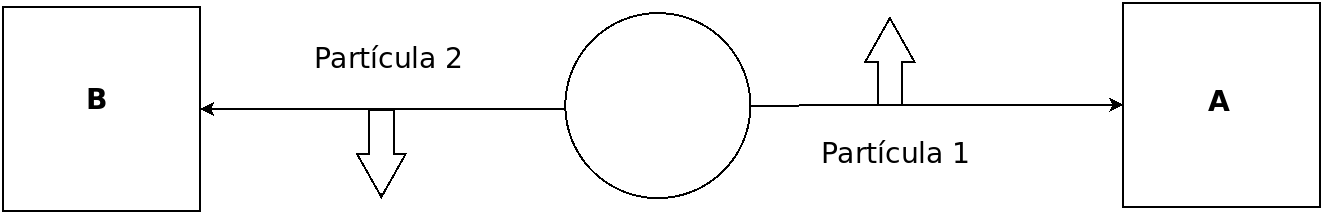
\includegraphics[scale=0.27]{./spin_correlation_spin_singlet.png} 
\end{center} 
\caption{Correlación de spin para un estado \textit{spin-singlet}}
\label{fig::spin_correlation_spin_singlet}
\end{figure}
Para un sistema de una partícula de spin $\frac{1}{2}$ se tienen los  eigenkets(vectores propios) $S_x$ y $S_z$ están relacionados de la siguiente manera \footnote{ver\ref{sec::appendix} o \cite{Sakurai}}
\begin{equation}
|\mathbf{\hat{x}\pm}\rangle=\frac{1}{\sqrt{2}}\big (|\mathbf{\hat{z}+}\rangle \pm |\mathbf{\hat{z}-}\rangle  \big),\,\,\,\,\,|\mathbf{\hat{z}\pm}\rangle=\frac{1}{\sqrt{2}}\big (|\mathbf{\hat{x}+}\rangle \pm |\mathbf{\hat{x}-}\rangle  \big).
\end{equation}
Continuando la discusión con el sistema compuesto, se puede reescribir el estado de spin-singlet \ref{eq::singlet_state} escogiendo al eje $x$ cómo eje de cuantización de la siguiente manera:
\begin{equation}
|\text{\textit{spin-singlet}}\rangle=\frac{1}{\sqrt{2}}\big( |\mathbf{\hat{x}}-;\mathbf{\hat{x}}+\rangle -|\mathbf{\hat{x}}+;\mathbf{\hat{x}}-\rangle  \big).
\end{equation}
está expresión es muy parecida a \ref{eq::singlet_state} y aparte del signo(que es una convención) se pudo esperaba tener una expresión análoga debido al hecho que para los estados de \textit{spin-singlet} no hay preferencia de dirección espacial. Suponiendo ahora que el observador A puede elegir medir $S_z$ or $S_x$ para la partícula 1 al cambiar la orientación de su dispositivo para medir el spin, mientras que el observador B se concentra en una sola dirección $S_x$ para la partícula 2. Si A mide $S_z$ y obtiene un valor positivo B tiene claramente $50\%-50\%$ chance de hallar $S_x\, +$ o $S_x\,-$ aunque se sepa que $S_z$ es con certeza negativo, su componente $S_x$ está totalmente indeterminado. Por el otro lado, suponiendo que A escoge medir $S_x$ entonces cuando mida un valor positivo para la partícula 1 el observador B tendrá con certeza un valor negativo para $S_x$. La última opción en la que el observador A prefiere no hacer ninguna medición sobre la partícula 1 entonces es claro que el observador B tiene de nuevo $50\%-50\%$ chance de medir $S_x\,+$ o $S_x\,-$, para resumirlo
\begin{enumerate}
\item Si A mide $S_z$ y B mide $S_x$, entonces hay una correlación completamente aleatoria entre las dos mediciones. 
\item Si A mide $S_x$ y B mide $S_x$, entonces hay una correlación perfecta(signos opuestos en las mediciones) entre las dos mediciones.
\item Si A no realiza medición, entonces las mediciones de B dan resultados aleatorios.
\end{enumerate}
Estos hechos demuestran que el resultado de la medición realizada por B parece depender de que tipo de medición el observador decide hacer: una medición de $S_x$, una medición de $S_y$, o ninguna medición. Es importante recalcar que A y B pueden estar ha kilómetros de distancia sin posibilidad de comunicación o alguna interacción. El observador A puede decidir la orientación de su dispositivo para medir el spin mucho después de que las partículas se separan. Pareciera ser que la partícula 2 ''sabe'' el componente del spin de la partícula 1 que se está midiendo instantáneamente. \\
La interpretación ortodoxa(la interpretación de Copenhagen) de está situación es la siguiente, la medición del observador A es un proceso de selección o filtrado. Cuando se mide $S_z$ de la partícula 1 y se obtiene un valor positivo, entonces se selecciona al componente $|\mathbf{\hat{z}}+;\mathbf{\hat{z}}-\rangle$ o la función de onda colapsa a este estado, una medición subsecuente de $S_z$ en la otra partícula tan sólo confirma que el estado es de hecho $|\mathbf{\hat{z}}+;\mathbf{\hat{z}}-\rangle$ o sigue en este estado. Se debe aceptar que lo que parece ser una medición en una parte del sistema es una medición en el sistema bipartito o el sistema completo.
\subsection{Principio de localidad de Einstein y la desigualdad de Bell}
Varios físicos han tenido una inconformidad o han tenido otras interpretaciones con respecto a la interpretación ortodoxa antes expuesta. Probablemente el más famoso siendo Albert Einstein que siempre mostró e hizo explícita su inconformidad con varios aspectos de la teoría cuántica. El principio de localidad de Einstein es el siguiente: La situación real es que el comportamiento del sistema $S_2$ es independiente del sistema $S_1$ que esta espacialmente separado del primer sistema y por lo tanto no tiene una influencia directa. Este problema fue discutido por primera vez en un artículo seminal que se conoce como la paradoja EPR(Einstein, Podolsky y Rosen) ver \cite{Einstein}. Algunos han argumentado que las dificultades o incongruencias encontradas en este fenómeno son inherentes de las interpretaciones probabilísticas de la mecánica cuántica y que el comportamiento de la dinámica a nivel microscópico aparenta ser probabilístico debido a que se desconocen algunos parámetros por descubrir que se han llamado \textbf{variables ocultas}(\textit{hidden variables}) no han sido especificados. Hay varias propuestas teóricas alternativas a la interpretación ortodoxa de la mecánica cuántica basadas en variables ocultas u otras consideraciones, por ejemplo la teoría de onda piloto de Bohm, introducida por uno de los padres de la teoría cuántica, Louis de Broglie. La pregunta fundamental para establecer la validez de la teoría cuántica es, ¿las teorías alternativas hacen predicciones que difieren de las hechas por la mecánica cuántica?. Hasta 1964 se creía que las teorías alternativas podían manipularse de tal forma que sus predicciones siempre coincidían  con las predicciones cuánticas, el debate se podía considerar en ese sentido un tópico metafísico o filosófico, al final los resultados experimentales eran idénticos. No fue hasta que John. S. Bell dedujo que las teorías alternativas basadas en el principio de localidad de Einstein producían predicciones en la forma de una relación de desigualdad entre los observables de experimentos de correlaciones de spin que estaba en desacuerdo con las predicciones para el mismo experimento derivadas de la interpretación ortodoxa de la mecánica cuántica que además podía ser sometida a confirmación experimental.\\
Aquí se derivan la relación de desigualdad de Bell en el marco de un modelo simple concebido inicialmente por Eugene Wigner, que incorporar todos los aspectos fundamentales de las teorías alternativas basadas en las variables ocultas. 
\section{Apéndice}\label{sec::appendix}
\begin{thebibliography}{99}
%% La bibliografía se ordena en orden alfabético respecto al apellido del 
%% autor o autor principal
%% cada entrada tiene su formatado dependiendo si es libro, artículo,
%% tesis, contenido en la web, etc
\bibitem{Arfken} George Arfken. \textit{Mathematical Methods for Physicists}.

\bibitem{Bell} J.S. Bell. \textit{On the Einstein Podolski Rosen Paradox}. \url{https://cds.cern.ch/record/111654/files/vol1p195-200_001.pdf}

\bibitem{Clauser} John F. Clauser, Michael A. Horne, Abner Shimony, Richard Holt. \textit{PROPOSED EXPERIMENT TO TEST LOCAL HIDDEN-VARIABLE THEORIES.}. Physical Review Letters,. 23(15):880-4, \url{https://journals.aps.org/prl/abstract/10.1103/PhysRevLett.23.880}.

\bibitem{Einstein} Einstein A., B. Podolsky, N. Rosen, \textit{Can Quantum-Mechanical Description of Physical Reality be Considered Complete?}. Physical Review. \url{doi:10.1103/PhysRev.47.777}

\bibitem{Medina} J. Medina. \textit{Reporte de Seminario 1. Computación Cuántica}. \url{https://github.com/Julio-Medina/Seminario/blob/main/Reporte_final/reporte_final.pdf}

\bibitem{Nielsen} Michael A. Nielsen, Isaac L. Chuang. \textit{Quantum Computation adn Quantum Information}. Cambridge University Press 2010. 10th. Anniversary Edition.

\bibitem{Feynman} Richard P. Feynman. \textit{Simulating Physics with Computers.} \url{https://doi.org/10.1007/BF02650179}.

\bibitem{Qiskit} \textit{Qiskit Textbook}. \url{https://qiskit.org/textbook-beta}

\bibitem{Mermin} N. David Mermin \textit{Quantum Computer Science: An Introduction}. Cambridge University Press, 2007.

\bibitem{Sakurai} J.J. Sakurai \textit{Modern Quantum Mechanics}. The Benjamin/Cummings Publishing Company, 1985.

\bibitem{Dotsenko} Viktor Dotsenko. \textit{An Introduction to the Theory of Spin Glasses and Neural Networks}. World Scientific 1994.

\bibitem{Bahri} Yasaman Bahri, Jonathan Kadmon, Jeffrey Pennington, Sam S. Schoenholz, Jascha Sohl-Dickstein, Surya Ganguli. \textit{Statistical Mechanics of Deep Learning}. \url{https://www.annualreviews.org/doi/pdf/10.1146/annurev-conmatphys-031119-050745}

\bibitem{openQASM} OpenQASM. \url{https://github.com/openqasm/openqasm}.
 

\end{thebibliography}
\end{document}

